Kuvassa \ref{oauth} on tunnistautumisprotokollien sekvenssikaavio, jossa on kuvattu vaiheet käyttäjän kirjautuessa web-sivulle. Useimmat vaiheista tapahtuu käyttäjältä näkymättömissä selaimen uudelleenohjauksella. Käyttäjälle näkyvät vaiheet ovat 4 ja 5, joissa käyttäjältä pyydetään käyttäjätunnus sekä salasana ja varmistetaan tietojen lähetys web-palveluun. Vaiheet on kuvattu aiemmassa kuvassa \ref{facebook_login}.

\begin{figure}[ht]
\centering
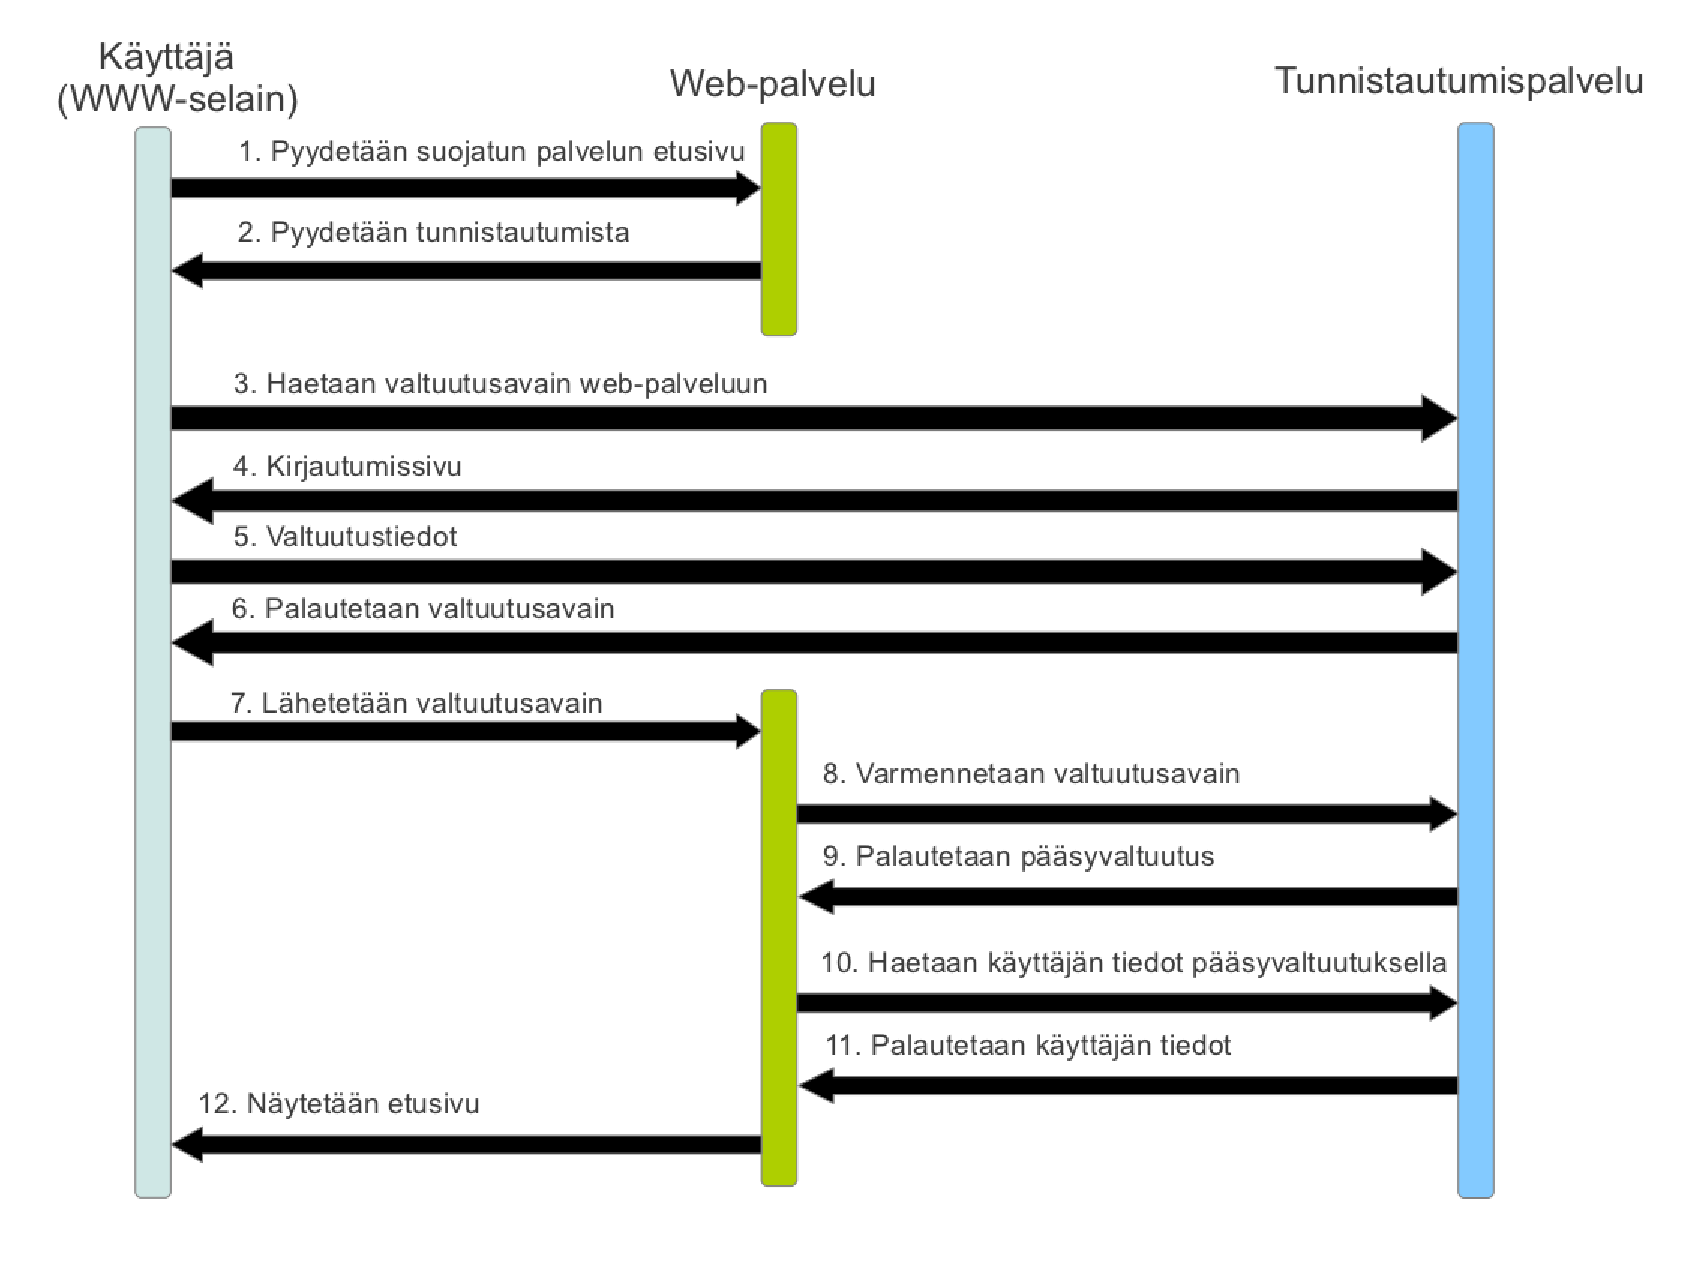
\includegraphics[width=\textwidth]{teknologiat/protokollat/oauth.eps}
\caption{Tunnistautuminen sekvenssikaaviona}%
\label{oauth}
\end{figure}

Tunnistautumisprotokollia tutkitaan ja kehitetään monen eri tahon toimesta. Web Services -teknologioita standardoinut OASIS (Organization for the Advancement of Structured Information Standards) on kehittänyt XML-pohjaista SAML-kieltä, Microsoftilla on oma Windows Live ID -standardinsa ja avoimen lähdekoodin maailmassa on syntynyt OpenID \cite{open_identity}.

Windows Live ID on osittain suljettu standardi, joka tarjoaa tunnistautumisprotokollien lisäksi täydellisen keskitetyn käyttäjän identiteetin hallinnan \cite{open_identity}. Toteuttava protokolla silmälläpitäen tämä ei ole kiinnostavaa, koska toteutettavassa prototyypissä on tarkoitus käyttää organisaatioiden nykyisiä käyttäjänhallintajärjestelmiä (esim. LDAP) hyväksi.

Prototyyppiin valittavien teknologiaratkaisujen yksi peruste on avoimuus. Käytettyjen teknologioiden tulee olla avoimia, jotta niiden toiminta tunnetaan mahdollisimman hyvin. Tässä valossa kiinnostavia protokollia on SAML sekä OpenID ja sen rinnalla kulkeva OAuth. Sekä SAML:ia että OpenID:tä ja OAuthia käsitellään seuraavissa alaluvuissa, joissa arvioidaan niiden käyttöä prototyypin toteutuksessa.